\de{ĐỀ THI HỌC KỲ II NĂM HỌC 2022-2023}{THPT Nguyễn Hữu Cảnh}

\begin{center}
	\textbf{PHẦN 2 - TỰ LUẬN}
\end{center}

\begin{bt}%[0T7B1-2]%[Dự án đề kiểm tra HKII NH 22-23-TheHung Nguyên]%[Trường Nguyễn Hữu Cảnh]
		Giải bất phương trình $-x^2+x+2\geq 0$.
	\loigiai{Ta có $-x^2+x+2= 0\Leftrightarrow \hoac{& x=-1 \\ & x=2.}$\\
		Bảng xét dấu. 
		\begin{center}
				\begin{tikzpicture}[font=\normalsize,t style/.style={style=solid}]
				\tkzTabInit[nocadre=false,lgt=3,espcl=2,deltacl=0.5]
				{$x$ /1, $-x^2+x+2$/0.75}
				{$ -\infty $,$ -1 $,$2 $,$ +\infty $}
				\tkzTabLine{  , -,0 , +,0  , -,  }  
			\end{tikzpicture}
		\end{center}
Dựa vào bảng xét dấu, tập nghiệm của bất phương trình $-x^2+x+2\geq 0$ là $S=[-1;2]$.
	}
\end{bt}

\begin{bt}%[0T7B1-2]%[Dự án đề kiểm tra HKII NH 22-23-TheHung Nguyên]%[Trường Nguyễn Hữu Cảnh]
		Tìm $m$ để biểu thức $f(x)=(m+1)x^2+4(m-1)x+3m-3>0$ luôn đúng với mọi $x\in\mathbb{R}$.
	\loigiai{
		\begin{itemize}
			\item Với $m+1=0\Leftrightarrow m=-1$, khi đó $f(x)=-8x-6>0\Leftrightarrow x<-\dfrac{3}{4}$ không thỏa với $\forall x\in \mathbb{R}$.
			\item $f(x)>0, \forall x \in \mathbb{R}\Leftrightarrow\heva{& a>0 \\ & \Delta<0}\Leftrightarrow \heva{& m>-11 \\ & 16(m-1)^2-4(m+1)(3m-3)<0}\Leftrightarrow\heva{& m>-1 \\ & m<7.}$
		\end{itemize}
	Vậy $m\in (-1;7)$ thì thỏa đề bài.
	}
\end{bt}

\begin{bt}%[0T8B2-1] %[Dự án đề kiểm tra HKII NH 22-23-TheHung Nguyên]%[Trường Nguyễn Hữu Cảnh]
		Từ các chữ số $1$, $2$, $3$, $4$, $5$, $6$, $7$ có thể lập được bao nhiêu số tự nhiên có $5$ chữ số khác nhau và bắt đầu bởi chữ số $3$.
	\loigiai{Gọi số cần tìm có dạng $\overline{abcd}$ được lập từ các số $1$, $2$, $3$, $4$, $5$, $6$, $7$.
		\begin{itemize}
			\item Vì bắt đầu bởi chữ số $3$ nên $a$ có $1$ cách chọn.
			\item Xếp các vị trí còn lại có $\mathrm{A}_8^4$ cách chọn.
		\end{itemize}
	Vậy có $1\cdot \mathrm{A}_8^4=360$ số.
	}
\end{bt}

\begin{bt}%[0T8B2-2]%[Dự án đề kiểm tra HKII NH 22-23-TheHung Nguyên]%[Trường Nguyễn Hữu Cảnh]
		Có $5$ cuốn sách Toán khác phau, $6$ cuốn sách Lý khác nhau và $3$ cuốn sách Hóa khác nhau. Hỏi có bao nhiêu cách chọn ra hai cuốn sách khác loại?
\loigiai{
	\begin{itemize}
		\item Chọn $1$ sách Toán, $1$ sách Lý có $5\cdot 6=30$ cách. 
		\item Chọn $1$ sách Toán, $1$ sách Hóa có $5 \cdot 3=15$ cách. 
		\item Chon $1$ sách Lý, $1$ sách Hóa có $6 \cdot 3=18$ cách.
	\end{itemize}
 		Vậy có $30+15+18=63$ cách chọn.
	}
\end{bt}

\begin{bt}%[0T8B2-2]%[Dự án đề kiểm tra HKII NH 22-23-TheHung Nguyên]%[Trường Nguyễn Hữu Cảnh]
		Cho hàng ghế dài gồm $9$ ghế đánh số từ $1$ đến $9$. Tìm số cách xếp $4$ nam và $5$ nữ vào hàng ghế này sao cho $3$ nam ngồi ở các vị trí $1$, $2$, $3$.
\loigiai{
		\begin{itemize}
		\item 	Số cách chọn $3$ nam trong $4$ nam xếp vào $3$ vị trí đầu tiên có $\mathrm{A}_4^3$ cách.
		\item  Xếp $6$ người còn lại vào $6$ vị trí trống có $6!$ cách.	
	\end{itemize}
	Vậy có  $\mathrm{A}_4^3 \cdot 6!=24\cdot720=17280$ cách. 
	}
\end{bt}

\begin{bt}%[0T0B2-3]%[Dự án đề kiểm tra HKII NH 22-23-TheHung Nguyên]%[Trường Nguyễn Hữu Cảnh]
		Một bình hoa gồm $6$ bông màu trắng, $7$ bông màu đỏ và $5$ bông màu vàng (các bông hoa khác nhau), lấy ngẫu nhiên ra $5$ bông hoa. Tính xác suất để lấy ra $5$ bông hoa cùng màu.
\loigiai{Ta có $n(\Omega)=\mathrm{C}_{18}^5=8568$ cách.\\
	 Gọi $A$ là biến cố \lq\lq $5$ bông hoa cùng màu.\rq\rq
	 \begin{itemize}
	 	\item Trường hợp $1$: Cùng màu trắng có  $\mathrm{C}_6^5=6$ cách.
	 	\item Trường hợp $2$: Cùng màu đỏ có  $\mathrm{C}_7^5=21$  cách.
	 	\item Trường hợp $3$: Cùng màu vàng có $\mathrm{C}_5^5=1$ cách.
	 \end{itemize}
	Do đó  $n(A)=6+21+5=28$.\\
	Vậy xác suất biến cố $A$ là
	$ \mathrm{P}(A)=\dfrac{n(A)}{n(\Omega)}=\dfrac{28}{8568}=\dfrac{1}{306}$.	
}
\end{bt}





%%=====Bài 5
\begin{bt}%[Dự Án Đề Thi HK2-K10-2022-2023]%[Nguyễn Văn Sang]%[0D8B3-1]
Khai triển biểu thức $(2x-1)^5$ theo công thức khai triển nhị thức Newton.
\loigiai{
Khai triển nhị thức Newton của  $(2x-1)^5$, ta được
\begin{eqnarray*}
	(2x-1)^5&=&\mathrm{C}_5^0(2x)^5+\mathrm{C}_5^1(2x)^4(-1)^1+\mathrm{C}_5^2(2x)^3(-1)^2\\
	&& +\, \mathrm{C}_5^3(2x)^2(-1)^3+\mathrm{C}_5^4(2x)^1(-1)^4+\mathrm{C}_5^5(-1)^5\\
	        &=&32x^5-80x^4+80x^3-40x^2+10x-1.
\end{eqnarray*}
}
\end{bt}

%%=====Bài 6
\begin{bt}%[Dự Án Đề Thi HK2-K10-2022-2023]%[Nguyễn Văn Sang]%[0H9B2-5]
Trong hệ trục tọa độ $Oxy$, cho $\triangle ABC$ có $A(1;2)$, $B(-2;0)$, $C(4;-2)$.
\begin{enumerate}
	\item Viết phương trình tham số đường trung tuyến $AM$ của $\triangle ABC$.
	\item Tính khoảng cách từ điểm $A$ đến đường thẳng chứa cạnh $BC$.
\end{enumerate}
\loigiai{
\begin{enumerate}
	\item Viết phương trình tham số đường trung tuyến $AM$ của $\triangle ABC$.\\
	Gọi $M$ là trung điểm $BC$ suy ra $M(1;-1)$.\\
	Đường trung tuyến $AM$ đi qua $A(1;2)$ và nhận $\overrightarrow{AM}=(0;-3)$ làm một véc-tơ chỉ phương.\\
	Phương trình tham số đường thẳng $AM\colon \heva{& x=1 \\ & y=2-3t}, (t\in \mathbb{R})$.
	\item Tính khoảng cách từ điểm $A$ đến đường thẳng chứa cạnh $BC$.\\
	Đường thẳng $BC$ đi qua $B(-2;0)$ và nhận $\overrightarrow{BC}=(6;-2)$ làm một véc-tơ chỉ phương nên có một véc-tơ pháp tuyến là $\overrightarrow{n}_{BC}=(1;3)$.\\
	Phương trình tổng quát đường thẳng $BC$ là
	$$1(x+2)+3(y-0)=0\Leftrightarrow x+3y+2=0.$$
	Khoảng cách từ $A$ đến đường thẳng $BC$ là
	$$\mathrm{d}(A,BC)=\dfrac{|1+3\cdot2+2|}{\sqrt{1^2+3^2}}=\dfrac{9\sqrt{10}}{10}.$$
	
\end{enumerate}
}
\end{bt}

%%=====Bài 7
\begin{bt}%[Dự Án Đề Thi HK2-K10-2022-2023]%[Nguyễn Văn Sang]%[0H9B3-2]
Viết phương trình đường tròn $(C)$ có đường kính $AB$ với $A(1;1)$; $B(7;5)$.
\loigiai{
\immini
{
Gọi $I$ là tâm đường tròn đường kính $AB$.\\
Suy ra $I$ là trung điểm $AB$ và $I(4;3)$.\\
Ta có $\overrightarrow{IA}=(-3;-2)$ và bán kính  $R=IA=\sqrt{13}$.\\
Phương trình đường tròn đường kính $AB$ là 
$$ (C)\colon (x-4)^2+(y-3)^2=13.$$
}
{
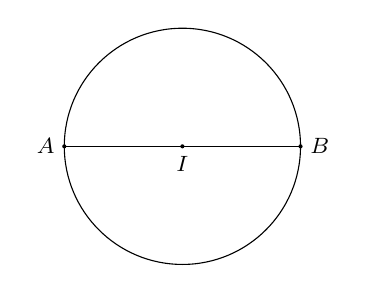
\begin{tikzpicture}[scale=.75, font=\footnotesize, line join=round, line cap=round, >=stealth]
	\draw (0,0) circle (2cm);
	\fill (-2,0) circle (1pt) node[left]{$A$};
	\fill (2,0) circle (1pt) node[right]{$B$};
	\fill (0,0) circle (1pt) node[below]{$I$}; 
	\draw (-2,0)--(2,0);
\end{tikzpicture}
}
}
\end{bt}
%%=====Bài 8
\begin{bt}%[Dự Án Đề Thi HK2-K10-2022-2023]%[Nguyễn Văn Sang]%[0H9K3-5]
	Trong mặt phẳng $Oxy$ cho đường tròn $(C)\colon x^2+y^2-2x+4 y-4=0$. Viết phương trình đường thẳng $\Delta$ song song với đường thẳng $d\colon 2 x-y+1=0$ và cắt đường tròn $(C)$ theo một dây cung có độ dài bằng $4$.
	\loigiai{
	\immini
	{
	Gọi $AB=\Delta \cap (C)$ và $H$ là trung điểm $AB$.\\
	Đường tròn $(C)$ có tâm $I(1;-2)$, bán kính $R=\sqrt{9}=3$.\\
	Đường thẳng $\Delta$ song song với $d\colon 2 x-y+1=0$ suy ra $\Delta$ có dạng $$\Delta\colon 2x-y+m=0, (m \neq 1).$$
	Khoảng cách từ $I$ đến $\Delta$ là $IH=\dfrac{|m+4|}{\sqrt{5}}$.\\
	Xét $\triangle IHA$ vuông tại $H$, ta có $IH^2=IA^2-AH^2=9-4=5$.
	}
	{
	\begin{tikzpicture}[scale=.75, font=\footnotesize, line join=round, line cap=round, >=stealth]
		\draw (0,0) circle (2cm);
		\coordinate (A) at ($(0,0)+(-135:2cm)$); 
		\coordinate (B) at ($(0,0)+(-45:2cm)$); 
		\fill (A) circle (1pt) node[left]{$A$};
		\fill (B) circle (1pt) node[right]{$B$};
		\fill (0,0) coordinate (I) circle (1pt) node[above]{$I$}; 
		\draw (A)--(B) (I)--++(-90:1.41) coordinate (H) circle (1pt) node[below]{$H$};
		\def\t{.2}\draw (H)--++(90:\t)--++(180:\t)--++(-90:\t); 
	\end{tikzpicture}
	}\noindent
	Suy ra 
	$$\dfrac{\left( m+4\right)^2}{5}=5\Leftrightarrow m^2+8m-9=0 \Rightarrow \hoac{& m=1 &\text{(loại)}\\& m=9 &\text{(nhận).}}$$
	Vậy $\Delta \colon 2x-y+9=0$.
	}
\end{bt}


